 %\pdfoutput=1
\documentclass[conference]{IEEEtran}
\IEEEoverridecommandlockouts
% The preceding line is only needed to identify funding in the first footnote. If that is unneeded, please comment it out.
\usepackage[T1]{fontenc}
\usepackage{cite}
\usepackage{mathtools}
\usepackage{stackengine}
\def\delequal{\mathrel{\ensurestackMath{\stackon[1pt]{=}{\scriptstyle\Delta}}}}
\usepackage{amsmath,amssymb,amsfonts}
\usepackage{amsmath,epsfig,cite,amsfonts,amssymb,psfrag,subfig}
\usepackage{graphicx}
\usepackage{textcomp}
\usepackage{xcolor}
\usepackage{algorithm}
\usepackage[noend]{algpseudocode}
\usepackage{amsthm}
\def\BibTeX{{\rm B\kern-.05em{\sc i\kern-.025em b}\kern-.08em
    T\kern-.1667em\lower.7ex\hbox{E}\kern-.125emX}}
\allowdisplaybreaks
\newtheorem{remark}{Remark}
\newtheorem{theorem}{Theorem}
\newtheorem{lemma}{Lemma}
\newtheorem{proposition}{Proposition}
\newtheorem{corollary}{Corollary}
\newcommand{\diag}{\mathop{\mathrm{diag}}}
\DeclareMathOperator{\E}{\mathbb{E}}
\usepackage[margin=0.7in]{geometry}
\setlength{\columnsep}{11mm}
\begin{document}

\title{Dynamic RB scheduling for different slices of eMBB and URLLC in the O-RAN system \vspace{-.1cm}
}
%
%\author{\IEEEauthorblockN{1\textsuperscript{st} Mojdeh Karbalaee Motalleb}
%\IEEEauthorblockA{\textit{Electrical and Computer Engineering} \\
%\textit{Tehran University}\\
%Tehran, Iran \\
%mojdeh.karbalaee@ut.ac.ir}
%\and
%\IEEEauthorblockN{2\textsuperscript{nd} Vahid Shah-Mansouri}
%\IEEEauthorblockA{\textit{Electrical and Computer Engineering} \\
%\textit{Tehran University}\\
%Tehran, Iran \\
%vmansouri@ut.ac.ir}
%\and
%\IEEEauthorblockN{3\textsuperscript{rd} Salar Nouri Naghadeh}
%\IEEEauthorblockA{\textit{Electrical and Computer Engineering} \\
%\textit{Tehran University}\\
%Tehran, Iran \\
%salar.nouri@ut.ac.ir}
%}
%%%%%  \author{
%%%%%    \IEEEauthorblockN{Mojdeh Karbalaee Motalleb}
%%%%%    \IEEEauthorblockA{School of ECE, College of Engineering, University of Tehran, Iran \\
%%%%%    Email: \{mojdeh.karbalaee\}@ut.ac.ir,
%%%%%    \vspace{-.2cm}
%%%%%  }
%%%%%  }

\maketitle

\begin{abstract}

\end{abstract}
\section{Introduction} 

\begin{figure*}
  \centering 
    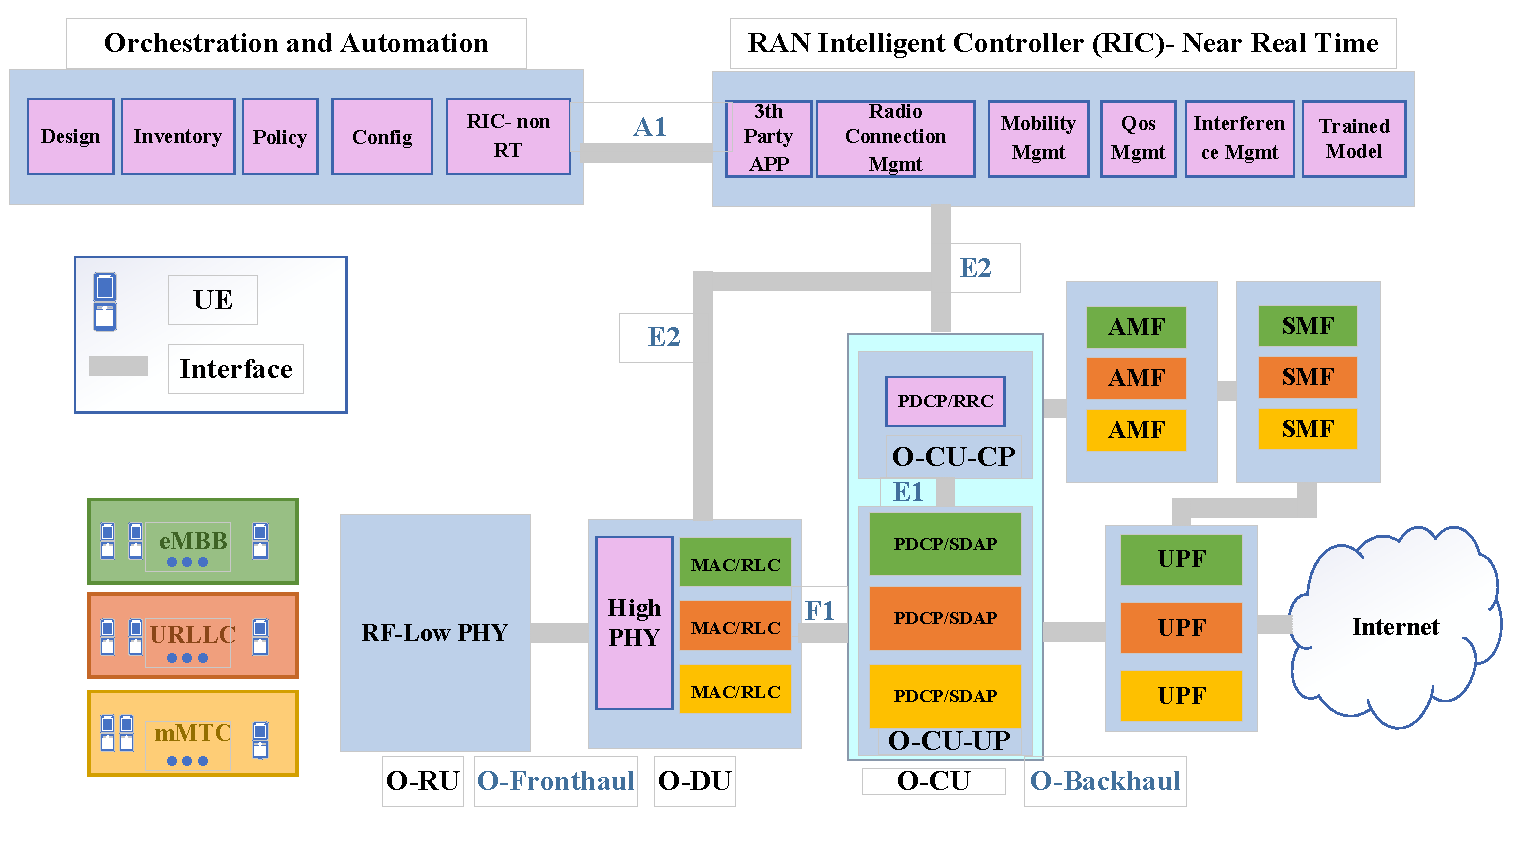
\includegraphics[scale = 0.5]{finalDraw.pdf}
    %\includegraphics[max height=30cm,max width=9.5cm]{Drawing15.eps}
    %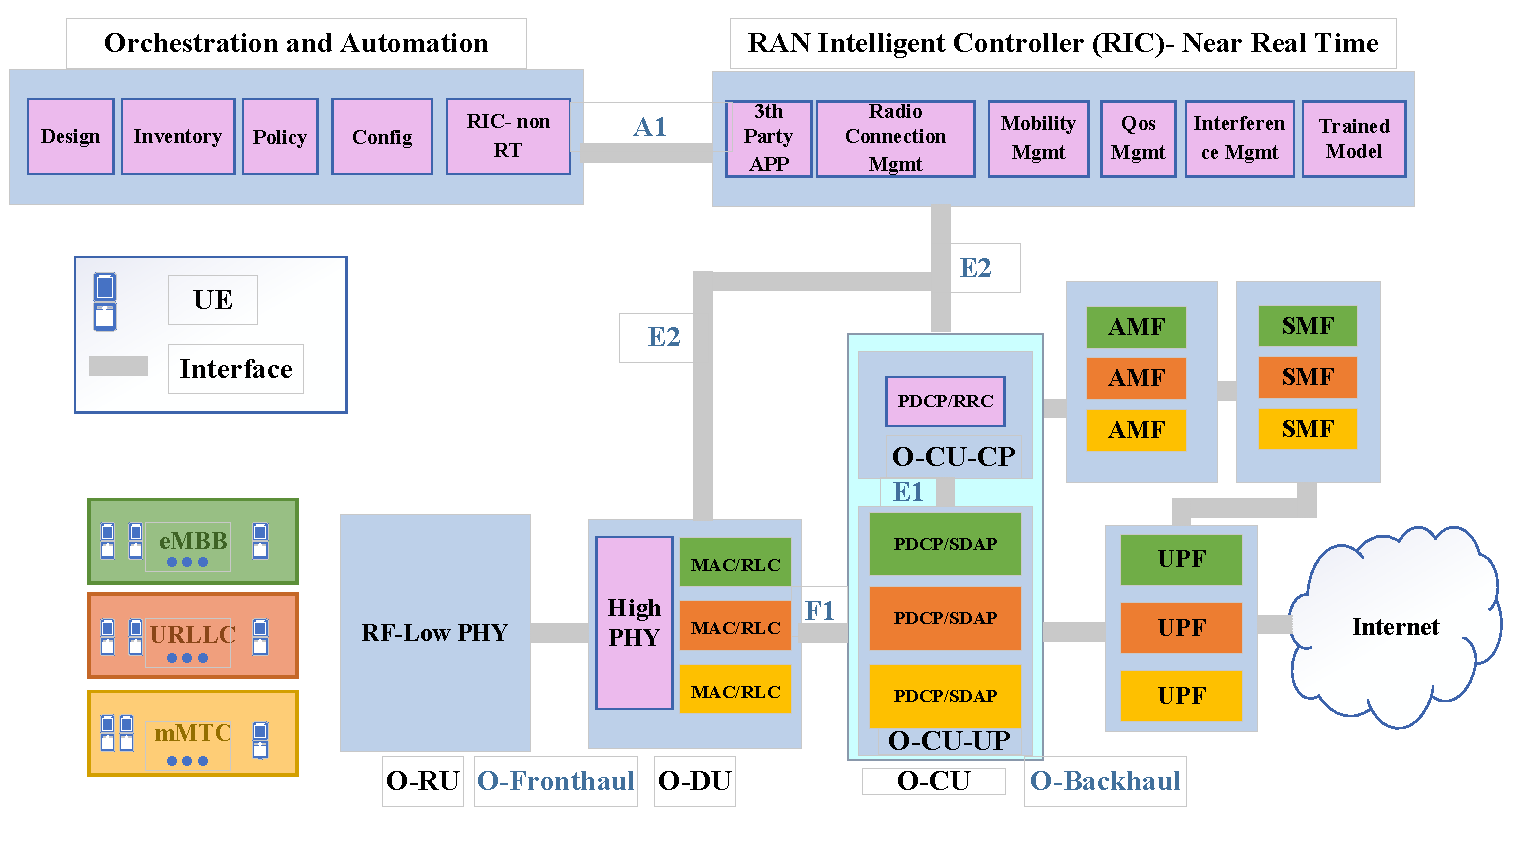
\includegraphics[width=\textwidth]{finalDraw.pdf}
  \caption{Network sliced ORAN system}
  \label{fig:1}
\end{figure*}

\section{System Model and Problem Formulation}
\subsection{System Model}
%This paper deals with the challenges of heterogeneous vehicular and cellular networks.
Assume we have two different services, namely, eMBB and URLLC; 
The system is serving a set of $\mathcal{U}_1$ eMBB single-antenna user equipments (UEs) and a set of $\mathcal{U}_2$ URLLC UEs.
Assume our system consists of $K$, preallocated physical resource blocks (PRBs). Moreover, the system considers to have $M_s^{d}$ VNFs for the processing of O-DU, $M_s^{c}$ VNFs for the processing of O-CU-UP of eMBB and URLLC ($ s \in \{1, 2\}$). 
Virtual network functions (VNFs) are functional blocks of the system. Each VNF instance runs on a virtual machine (VM) using resources from the data centers. 
Moreover, we assume there is a cell with one multi-antenna O-RU that serves UEs.
Furthermore, we suppose the channel distribution is known.
\subsection{The Achievable Rate}
The eMBB services typically use more than a one-time slot. But URLLC services use part of a time slot (mini-slot) since it has short packet transmission that it is indicated in Fig \ref{fig:2}. In addition, the URLLC must be punctured as soon as it has requested service as it requires very low latency.
\begin{figure}
  \centering 
    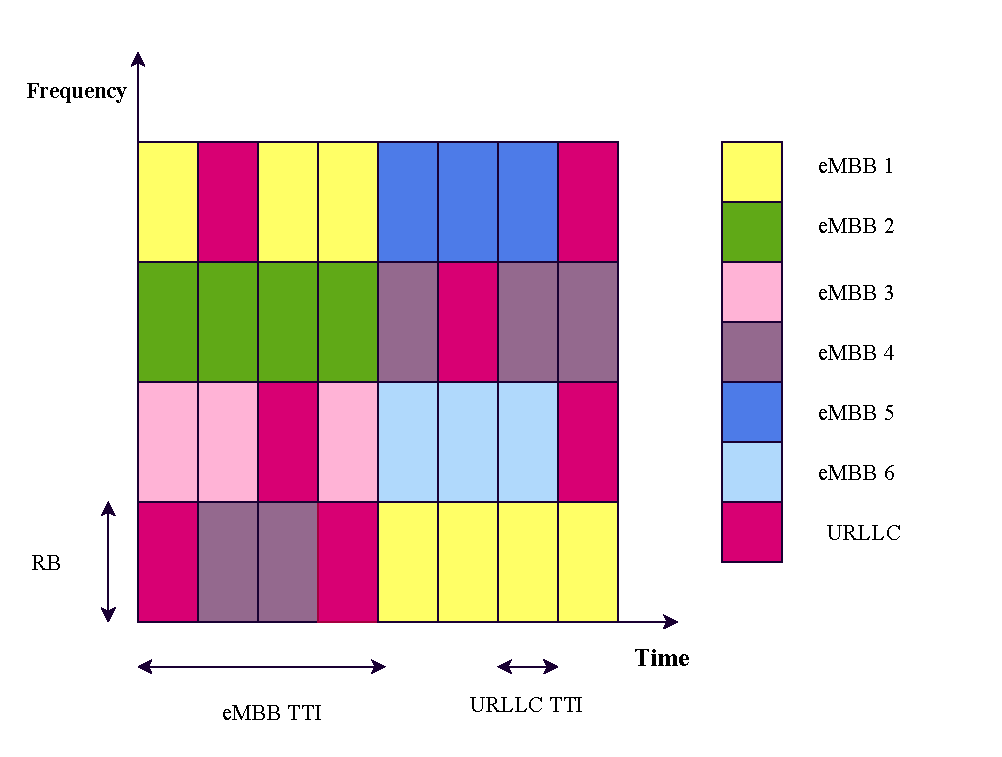
\includegraphics[scale = 0.4]{EU.pdf}
    %\includegraphics[max height=30cm,max width=9.5cm]{Drawing15.eps}
    %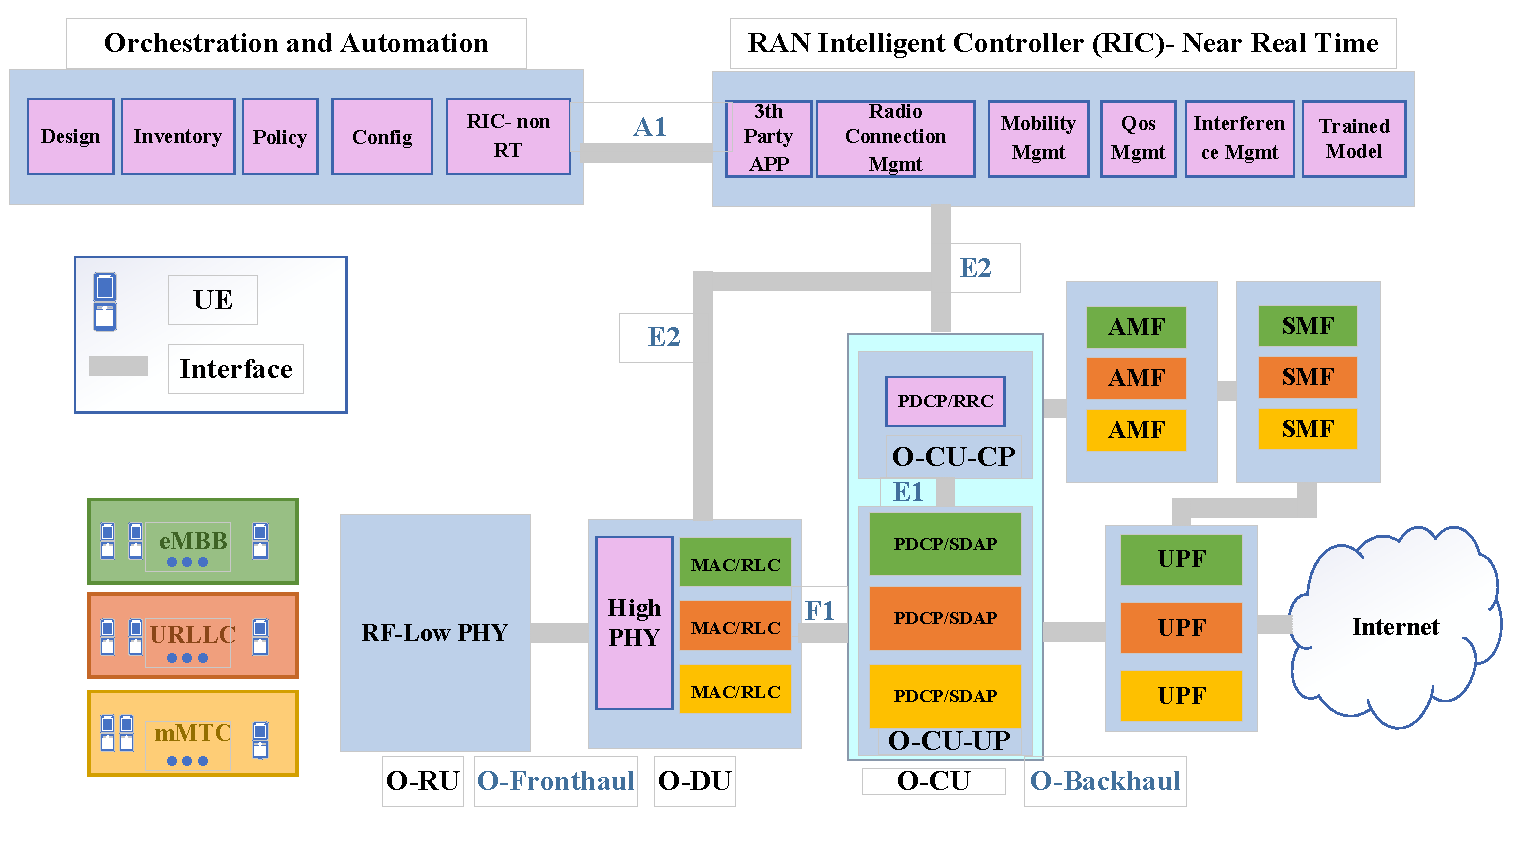
\includegraphics[width=\textwidth]{finalDraw.pdf}
  \caption{RB scheduling}
  \label{fig:2}
\end{figure}
Our current work allocates RBs to eMBB users at the beginning of each time slot using the PF principle, a scheduling strategy that balances throughput with fairness \cite{shi2022risk}.

The achievable data rate and the expectation of the achivable data rate for the $i^{th}$ UE request eMBB slice can be written as $\mathcal{R}_{i}^{e}(t)$, and $\bar{\mathcal{R}}_{i}^e(t)$, respectively.
\begin{equation}\label{eq1}
\begin{split}
\mathcal{R}_{i}^e(t) &= \sum_{k = 1}^K e^k_i(t) B (1-{n^k_i(t)}) \log_2({1+\frac{p^k_i(t)h^k_i(t)}{B \times N_0}}),\\
\bar{\mathcal{R}}_{i}^e(t) &= \E_{h}[\mathcal{R}_{i}^e(t)],
\end{split}
\end{equation}
where $B$ is the bandwidth of RBs. Also, $B\times N_0$ denotes the power of Gaussian additive noise. 
Moreover, $e^k_i(t)\in \{0,1\}$ is a binary variable that illustrates whether PRB $k$ is assigned to the $i^{th}$ eMBB UE or not. 
$p^k_i(t)$ represents the transmission power allocated by O-RU to $i^{th}$ UE of eMBB using PRB $k$.
$h^k_i(t)$ is the channel gain of a wireless link from 
O-RU to the $i^{th}$ eMBB UE using $k^{th}$ PRB which is Rayleigh fading.
Furthermore, $n^k_i(t)$ is the percentage of RB $k$ using eMBB $i$ that is punctuated by URLLC UEs is denoted as follows,
\begin{equation}
n^k_i(t) = \psi^k_i(t) \frac{\sum_{j \in \mathcal{U}_2}{\zeta}^u_{j}(t){\nu}^u \tau}{S_{max}(t)\tau},
\end{equation}
Where, $\psi^k_i(t)$ is the probability of puncturing eMBB UE $i$ using RB $k$.
Furthermore, ${\zeta}^u(t)$ is the arrival rate of URLLC UEs (arrival/slot/user).
Moreover, $\mathcal{U}_2$ is the set of URLLC UEs in the system.
In addition, $\nu^u$ is the URLLC packet size, and $\tau$ is the number of slot per second (slot/sec).
Assume the packet arrival of URLLC UEs follows a Poisson process with arrival rate $\lambda(t)$.
Therefore, the arrival data rate of URLLC $j$ is $\lambda_j(t) = {\zeta}^u_{j}(t){\nu}^u \tau$ .
Moreover, $S_{max}(t)$ is the flow density refers to how much data the system can handle for all URLLC users at any given time (bits/slot).
Moreover, we have $\sum_i e_i^k(t)\le 1$ to guarantee that each RB is allocated to a maximum of one eMBB UE.

Since the blocklength in URLLC is finite, the achievable data rate for the $j^{th}$ UE request in the URLLC service, is not achieved from Shannon Capacity formula. So, for the short packet transmission the achievable data rate and its expectation is written as follow, respectively, 
\begin{equation}\label{eq11}
\begin{split}
\mathcal{R}_{j}^u(t) &= \sum_{i = 1}^{U_1}\sum_{k=1}^K m_i^{k}(t) B \log_2({1+\frac{p^k_j(t)h^k_j(t)}{B \times N_0}})- \zeta_{j}^k(t)),\\
\bar{\mathcal{R}}_{j}^u(t) &= \E_{h}[\mathcal{R}_{j}^u(t)],
\end{split} 
\end{equation}
where $\zeta_{j}^k(t) = \log_2({e})Q^{-1}(\epsilon) \sqrt{\frac{C_{j}^k(t)}{N_{j}^k(t)}})$
where $\epsilon$ is the transmission error probability, $Q^{-1}$ is the inverse of Q function (i.e., Gaussian),
$C_{j}^k(t) = 1 - \frac{1}{(1+\rho_{j}^k(t))^2}$ depicts the channel dispersion of UE $j$ of URLLC, puncturing mini-slots of PRB $k$ and
$N_{j}^k(t)$ represents the blocklength of it. Moreover, $\rho_{j}^k(t)=\frac{p^k_j(t)h^k_j(t)}{B \times N_0}$ is the SNR of UE $j$ in URLLC service. 
Also, $m_i^{k}(t) $ is denoted as follow
\begin{equation}
m_i^{k}(t)= \frac{e_i^k(t)n^k_i(t)}{|\mathcal{U}_2|},
\end{equation}
where, $|\mathcal{U}_2|$ is the number of URLLC UEs in the system.
%The channel gain is assumed to be known with errors, the imperfection of channel estimation is
%modeled as follows
%\begin{equation}
%h^k_j(t) = \hat{h}^k_j(t) + \Delta h^k_j(t)
%\end{equation}
%Where, $\Delta h^k_j(t)$ denotes the estimation error with a Guassian distribution of
% \begin{equation}
%\Delta h^k_j(t)\backsim \mathcal{N}(0,\boldsymbol{\phi^k}^2),
%\end{equation}
\subsection{Mean Delay}
In this part, the mean processing delay for each service is obtained.
Suppose the mean total processing delay is depicted as $T_{\text{\text{tot}}}$,
\begin{subequations} 
\begin{alignat}{4}
T^{\text{tot}} &= T^{RU} + T^{\text{proc}},\\
T^{\text{proc}} &= T^{DU} + T^{CU}.
\end{alignat}
\end{subequations} 
We assume that the packet arrival rate of URLLC UEs follows a Poisson process with arrival rate $\lambda_{j}(t)$ for the $j^{th}$ UE.
Thus, we have $\lambda_j(t) = {\zeta}^u_{j}(t){\nu}^u \tau$.
Therefore, the mean arrival data rate of the O-CU-UP layer is $\alpha^C(t) = \sum_{j\in \mathcal{U}_2}\lambda_{j}(t)$.
Assume the mean arrival data rate for URLLC slice ($\alpha$) is approximately equal to the mean arrival data rate of the  the O-DU ($\alpha^D$). so $\alpha(t) = \alpha^C(t) \approx \alpha^D(t)$,
Because the amount of data traffic transferred along the route (regardless of frame changes) is constant.
Since, by using Burke’s theorem, the mean arrival data rate of the second layer, which are processed in the first layer, is still poisson with rate $\alpha$.
It is assumed that there are load balancers in each layer for each service to divide the incoming traffic to VNFs equally. %\cite{frdl,luong2018novel,luong2018novel1}.
Suppose the baseband processing of each VNF is depicted as M/M/1 processing queue.
Each packet is processed by one of the VNFs of a slice. So, the mean delay for the URLLC slice in the O-DU,and the O-CU is modeled as M/M/1 queue, is formulated as follows, respectively \cite{SystemCostMinimization,luong2018joint,luong2018novel},
\begin{equation}
\begin{split}
T^{DU} &= \frac{1}{\mu^d - \alpha(t)/{M^{d}(t)}},\\
T^{CU} &= \frac{1}{\mu^c - \alpha(t)/{M^{c}}(t)},\\
\end{split}
\end{equation}
where $M^{d}(t)$,and $M^{c}(t)$ are the variables that depict the number of VNFs in O-DU,and O-CU-UP, respectively. 
Moreover, $1/\mu^d$, and $1/\mu^c$ are the mean service time of the O-DU, and O-CU layers, respectively.
Besides, $\alpha$ is the  arrival rate which is divided
by load balancer before arriving to the VNFs. The arrival rate of each VNF in each layer for URLLC slice  is $\alpha/{M^{l}}$ $ l \in \{d,c\}$.

Suppose the mean transmission delay of the $j^{th}$ UE of the URLLC service on the wireless link is denoted by
$T_{j}^{RU}(t)$.
 Assume the arrival data rate of wireless link for each UE $j$ of URLLC service is $\lambda_j(t)$
As a result, we have $\sum_{j \in \mathcal{U}_2} \lambda_{j}(t) = \alpha(t)$.
Moreover, The service time of transmission queue for UE $j$ requesting URLLC service has
an exponential distribution with mean $1/R_{j}^u(t)$ and can be modeled as a M/M/1 queue \cite{SystemCostMinimization,luong2018joint,luong2018novel}.
 
Therefore, the mean delay of the transmission layer for UE $j$ in URLLC slice is
\begin{equation}
 T_{j}^{RU}(t) = \frac{1}{\bar{\mathcal{R}}_{j}^u(t) - \lambda_{j}(t)}.
\end{equation}


\subsection{Reliability of URLLC}
As we know, UEs request URLLC services, require services with low latency.
For the M/M/1 system, the probability of the delay for URLLC service in the O-RU is as follow, 
\begin{equation}
P_r\{T_{j}^{RU} \geq T_{RU}^{max}\} = e^{-(\bar{R}_{j}^u - \alpha)T_{RU}^{max}}
\end{equation} 
Also, we do not consider the reliability for O-CU and O-DU.

\subsection{Problem Statement}
%In this system, the goal is to minimize the cost of the system.
%The total power cost of O-RUs for transmitting data to UE is depicted as follow
%\begin{equation}
%P_{tot} = \sum_{r=1}^{R}P_r
%\end{equation}
In this paper, we strive to maximize the sum rate of all eMBB UEs and minimize the delay of URLLC UEs while imposing constraints on their performance based on their QoS.
The optimization problem is formulated as follow,

\begin{subequations} \label{mainP}
\begin{alignat}{4}
\max\limits_{ \boldsymbol{E}, \boldsymbol{\Psi},\boldsymbol{M} } &  \sum_i \bar{\mathcal{R}}_{i}^e(t) - \eta \sum_j T^{\text{tot}, u}(t)       \ \\
\text{subject to} \quad  & \bar{\mathcal{R}}_{i}^e(t) \geq  \mathcal{R}_{min}^e \quad \forall i \in \mathcal{U}_1, \label{p1} \\
& Pr\{\bar{\mathcal{R}}_{i}^e(t) \leq {R}_{min}^e\}  \leq \epsilon,\quad \forall i \in \mathcal{U}_1, \label{p2}\\
&T^{\text{tot}, u}_j(t)  \leq T_{min}^u  \quad \forall j \in \mathcal{U}_2, \label{p3} \\
&Pr\{T^{\text{RU}, u}_j(t) \geq T_{min}^u\} \leq \epsilon  \quad \forall j \in \mathcal{U}_2, \label{p4} \\
&\sum_{i=1}^{U_1}e^k_i(t)\leq 1 \quad \forall k \in \{1,...,K\},\label{p5} \\
&e^k_i(t)\in \{0,1\}  \quad \forall i,k, \label{p6} \\
& 0 \leq n^k_i(t)\leq 1  \quad \forall i,k, \label{p7} \\
& \mu^l \geq \alpha/M^l \quad l \in \{c,d\},\label{p8} \\
& \bar{\mathcal{R}}^u(t) \geq {\lambda}_{j}^u(t) \quad \forall j \in \mathcal{U}_2,\label{p9} \\
& 0 \leq M^l \leq M_{max}^l  \quad l \in \{c,d\},\label{p10}
\end{alignat}
\label{constraints}
\end{subequations}
Where, \eqref{p1}, guarantees the minimum data rate of eMBB UEs, also
\eqref{p2}, supports the reliability of eMBB while puncturing the URLLC. 
In addition, \eqref{p3}, and \eqref{p4} guarantee the latency and reliability of URLLC UEs, respectively.
Furthermore, eMBB RB allocation constraint is indicated by \eqref{p5}, and \eqref{p6}.
\eqref{p7}, indicate that the punctured mini-time slot are fewer than the total number of mini-slots in the RB.
\eqref{p8} and \eqref{p9} denotes the stability of the M/M/1 queue model.
\eqref{p10} restricts the number of VNF in each slice due to the limited resources.

\section{Proposed Algorithm}
In this section, we talk about our proposed algorithm to solve the problem \eqref{mainP}.
Since this problem is mixed-integer nonlinear programming (MINLP) with binary and integer variables, it is complicated to solve.

We can solve this problem on a two-time scale. On a large time scale, the problem of assigning RB to eMBB UEs is solved,
Also, in this time scale, we can estimate the optimal number of VNFs, and in the small time scale, the problem of URLLC puncturing is solved. 
\subsection{Large time scale}
In this time scale, we want to solve the problem of eMBB scheduling and finding the optimal number of VNF for URLLC UEs.
Here, we suppose the puncturing of URLLC is fixed, hence, we want to solve the problem \eqref{mainP}.
The problem \eqref{mainP}, is altered to the following problem


\begin{subequations} \label{mainP1}
\begin{alignat}{4}
\max\limits_{ \boldsymbol{E},\boldsymbol{M} } &  \sum_i \bar{\mathcal{R}}_{i}^e(t) - \eta T^{\text{proc}, u}(t)       \ \\
\text{subject to} \quad  & \bar{\mathcal{R}}_{i}^e(t) \geq  \mathcal{R}_{min}^e \quad \forall i \in \mathcal{U}_1, \label{p1} \\
& Pr\{\bar{\mathcal{R}}_{i}^e(t) \leq {R}_{min}^e\}  \leq \epsilon,\quad \forall i \in \mathcal{U}_1, \label{p12}\\
&\sum_{i=1}^{U_1}e^k_i(t)\leq 1 \quad \forall k \in \{1,...,K\},\label{p15} \\
&e^k_i(t)\in \{0,1\}  \quad \forall i,k, \label{p16} \\
& 0 \leq n^k_i(t)\leq 1  \quad \forall i,k, \label{p17} \\
& \mu^l \geq \alpha/M^l \quad l \in \{c,d\},\label{p18} \\
& 0 \leq M^l \leq M_{max}^l  \quad l \in \{c,d\},\label{p110}
\end{alignat}
\label{constraints}
\end{subequations}

Generally, let's assume O-CU and O-DU use the same processor. 
Consequently, the formulation becomes simpler. Despite this, the formulation remains the same, and the problem can still be solved similarly. 
Consequently, we have $\mu = \mu^c \approx \mu^d $. Additionally, the mean arrival data rate for the O-DU layer ($\alpha^C$) is the same as the O-CU-UP layer ($\alpha^C$). So $\alpha = \alpha^C \approx \alpha^D$. 
Accordingly, we can have $M^d(t) = M^c(t)$. Therefore, $T^{DU} = T^{CU}$, and $T^{proc} =2\times T^{DU}$.

The problem \eqref{mainP1}, is still mixed integer non-linear programming (MINP). Here, the problem \eqref{mainP1}
can also be decomposed into two sub-problems which is depicted as follow.
\subsubsection{sub-problem 1}
In this section, we want to solve the sub-problem of RB allocation of eMBB UEs.
The problem can be written as follow.
\begin{subequations} \label{mainP11}
\begin{alignat}{4}
\max\limits_{ \boldsymbol{E} } &  \sum_i \bar{\mathcal{R}}_{i}^e(t)       \ \\
\text{subject to} \quad  & \bar{\mathcal{R}}_{i}^e(t) \geq  \mathcal{R}_{min}^e \quad \forall i \in \mathcal{U}_1, \label{p11} \\
&\sum_{i=1}^{U_1}e^k_i(t)\leq 1 \quad \forall k \in \{1,...,K\},\label{p115} \\
&e^k_i(t)\in \{0,1\}  \quad \forall i,k, \label{p116} 
\end{alignat}
\label{constraints}
\end{subequations}
\subsubsection{sub-problem 2}
In this section, we want to solve the sub-problem of finding the optimal number of VNF for URLLC services.
The problem is formulated as follow.
\begin{subequations} \label{mainP2}
\begin{alignat}{4}
\min\limits_{ \boldsymbol{M} } &  T^{\text{proc}, u}(t)       \ \\
\text{subject to} \quad  & \mu^l \geq \alpha/M^l \quad l \in \{c,d\},\label{p28} \\
& 0 \leq M^l \leq M_{max}^l  \quad l \in \{c,d\},\label{p210}
\end{alignat}
\label{constraints}
\end{subequations}
\subsection{Small time scale}
In the small time scale, we assume that the eMBB RB allocation is performed and the optimal number of VNF for URLLC is obtained. Therefore, the problem of puncturing URLLC UEs is performed.
\begin{subequations} \label{mainP2}
\begin{alignat}{4}
\min\limits_{  \boldsymbol{\Psi} } &  \sum_j T^{RU, u}(t)       \ \\
\text{subject to} \quad  &T^{\text{tot}, u}_j(t)  \leq T_{min}^u  \quad \forall j \in \mathcal{U}_2, \label{p33} \\
& Pr\{\bar{\mathcal{R}}_{i}^e(t) \leq {R}_{min}^e\}  \leq \epsilon,\quad \forall i \in \mathcal{U}_1, \label{p32}\\
&Pr\{T^{\text{RU}, u}_j(t) \geq T_{min}^u\} \leq \epsilon  \quad \forall j \in \mathcal{U}_2, \label{p34} \\
& 0 \leq n^k_i(t)\leq 1  \quad \forall i,k, \label{p37} \\
& \bar{\mathcal{R}}^u(t) \geq {\lambda}_{j}^u(t) \quad \forall j \in \mathcal{U}_2,\label{p39} 
\end{alignat}
\label{constraints}
\end{subequations}



\bibliographystyle{IEEEtran}
\bibliography{ref}
\end{document} 